\chapter{Implementação do Processo}

A execução do processo ocorre por meio de componentes para a análise de similaridade, persistência dos dados, geração do alinhamento, lógica entre as etapas e utilitários para manipulação de dados (ver Figura \ref{fig:componentes}). Alguns componentes foram reusados, como o de similaridade léxica, que contém vários algoritmos para detectar a similaridade entre textos. Outros componentes foram desenvolvidos, como os responsáveis pela detecção da similaridade de recurso, alinhamento e outros.

\begin{figure}[!ht]
	\centering
	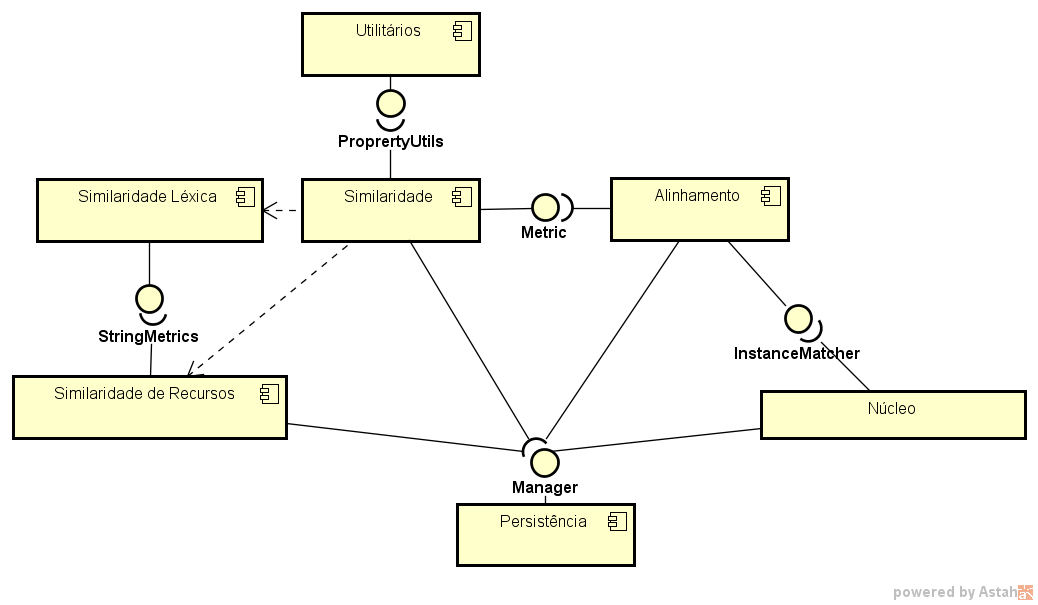
\includegraphics[width=0.9\textwidth]{./imagens/componentes.png}
    \caption{Componentes utilizados na implementação do processo}
	\label{fig:componentes}
\end{figure}

Apesar de existirem diversas soluções que contém algoritmos para o cálculo de similaridade e alinhamento entre recursos, optou-se pelo desenvolvimento de uma abordagem que contemplasse problemas provenientes de bases de dados reais (acentuação, ausência de propriedades, formatação e outros) \cite{castano2011ontology,ferrara2008towards}.
Os principais componentes utilizados são:

\section{Persistência}
O componente de persistência é responsável pelo acesso à base de conhecimento. Assim, é responsável por armazenar e recuperar os recursos e os alinhamentos que são utilizados ao longo do processo. Além disso, o mesmo atua como abstração do servidor de triplas (Virtuoso, OWLim etc.). Isso permite que o alinhamento seja executado diretamente nos datasets.

\section{Similaridade}
O componente de similaridade é dividido em dois subcomponentes, sendo eles o de similaridade léxica e recurso. O primeiro utiliza métricas que analisam a similaridade entre palavras e textos. Algumas dessas técnicas são Levenshtein \cite{levenshtein1966binary}, Cosseno \cite{singhal2001modern}, Jaro-Winkler \cite{winkler1990string} e outros. O segundo componente, que se refere à similaridade de recurso, utiliza o primeiro e tem como função gerar a similaridade entre recursos.

Para o cálculo da similaridade dos recursos foi utilizada uma abordagem baseada na técnica de subgrafo semântico \cite{wang2008lily}. Na prática, um subgrafo semântico diz respeito às triplas que estão relacionadas a um recurso qualquer, que estão de acordo com a modelagem ontológica. A Figura \ref{fig:subgrafo} representa um subgrafo que relaciona um autor e sua publicação. Além de propriedades de objetos, um subgrafo também possui propriedades de dados, tanto do recurso principal (Author), quanto dos conceitos relacionados (Production). % O trecho de código \ref{lst:similaridade} descreve a implementação do cálculo de similaridade.

\begin{figure}[!ht]
	\centering
	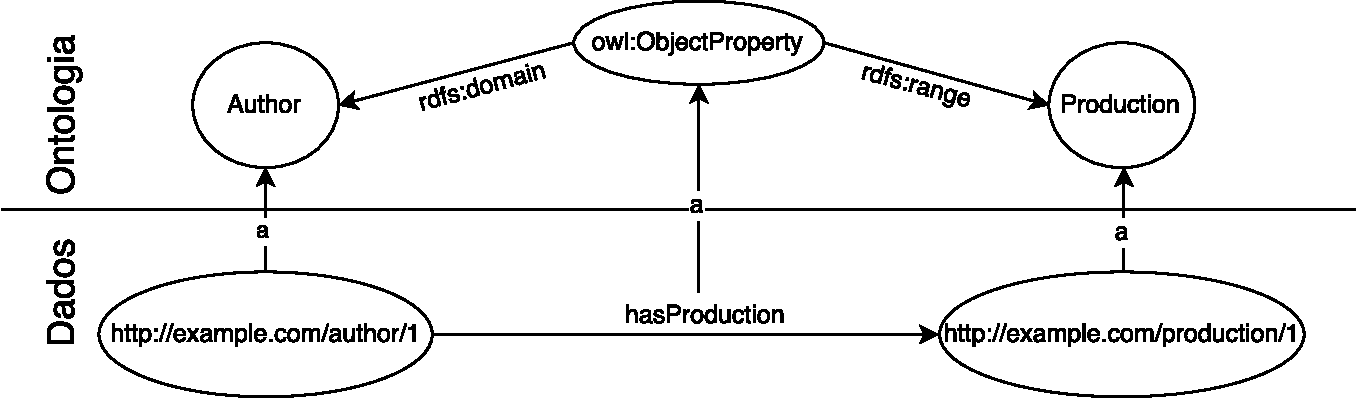
\includegraphics[width=0.9\textwidth]{./imagens/subgrafo_semantico.pdf}
    \caption{subgrafo que relaciona os conceitos Author e Publication}
	\label{fig:subgrafo}
\end{figure}

% \begin{lstlisting}[captionpos=b, caption= Trecho de código java para calcular a similaridade entre recursos, label=lst:similaridade,
%    basicstyle=\ttfamily,frame=single]
% float avg_similarity = 0;
% try {
%   //Gerando subgrafos
%   JSONObject graphA = resource1;
%   JSONObject graphB = resource2;

%   // Recuperando subgrafo com mais propriedades
%   if (graphA.length() > graphB.length()) {
%     JSONObject aux = graphA;
%     graphA = graphB;
%     graphB = aux;
%   }

%   // Numero de comparacoes internas
%   float innerComparisions = 0;

%   // Valor de similaridade para cada propriedade
%   float innerSimilaritySum = 0;

%   // Chaves de iteracao
%   Iterator keys = graphB.keys();

%   while (keys.hasNext()) {

%     //Recupera chave
%     String key = (String) keys.next();

%     // desconsiderando chaves que estiverem no set
%     if (propertySet != null && propertySet.contains(key)) continue;
%     try {

%       // Recuperando o valor da propriedade
%       Object pA = graphA.get(key);
%       Object pB = graphB.get(key);

%       // Casting para string
%       String propertyA = (pA instanceof JSONArray) ? ((JSONArray) pA).getString(0) : graphA.getString(key);
%       String propertyB = (pB instanceof JSONArray) ? ((JSONArray) pB).getString(0) : graphB.getString(key);

%       // Recuperando quantidade de tokens
%       int tokensizeA = propertyA.toString().split(" ").length;
%       int tokensizeB = propertyB.toString().split(" ").length;

%       //Similaridade temporaria
%       float tempSimirity = 0f;

%       // Recuperando Estrategia baseada na quantidade maxima de tokens
%       StringMetric metric1 = (StringMetric) MongeElkanMetricStrategy.getMetric(Math.max(tokensizeA, tokensizeB));

%       // Dispensando o tipo e a uri do recurso
%       if (key.equals("type") ||
%         key.equals("@id")) {
%         continue;

%         // Se for recurso
%     } else if (levels > 0 && propertyA.toLowerCase().contains("http://") && propertyB.toLowerCase().contains("http://")) {
%       innerComparisions++;
%       tempSimirity = this.compare(propertyA, propertyB, levels);

%       // Se for dado
%     } else {
%       innerComparisions++;
%       tempSimirity = metric1.compare(PropertyUtils.nameCleaning(propertyA, true), PropertyUtils.nameCleaning(propertyB, true));
%     }
%     System.out.println(key+" = "+tempSimirity);

%     // Atribuindo peso a similaridade
%     innerSimilaritySum+= tempSimirity * weight.getOrDefault(key,1f);
%   } catch (Exception e) {
%     continue;
%   }
% }

% // Definindo similaridade de recurso
% avg_similarity = innerSimilaritySum / innerComparisions;

% \end{lstlisting}


O valor gerado pelo componente de similaridade é enviado para o componente de alinhamento.
\section{Alinhamento}
O componente de alinhamento tem como responsabilidade determinar, de acordo com os valores obtidos na etapa de similaridade, se os recursos analisados realmente dizem respeito à mesma entidade do mundo real. Para determinar se o alinhamento deve ser realizado, este componente faz uso de limiares de aceitação, que são determinados previamente. Por esse motivo, o processo de alinhamento não é uma tarefa automática, pois precisa que os valores sejam ajustados. Existem diversas formas de determinar o valor do limiar, que vão desde executar várias vezes e analisar o melhor custo/benefício entre precisão e revocação até utilizar técnicas que atualizam o valor do limiar dinamicamente.


\section{Núcleo}
O componente de núcleo tem como principal função coordenar as atividades de alinhamento. Além de coordenar, é nesse componente que são definidos os limiares de aceitação, propriedades a serem desconsideradas, conceitos principais e conceitos relacionados, que servirão como parâmetro os componentes de alinhamento e similaridade.


\section{Utilitários}
O componente de utilitários tem como função realizar tratamentos nos textos que serão aplicados à função de similaridade. Alguns exemplos de tratamento são: tratamento de acentos, pontuação e outros.

